Cabe recalcar que el documento está inspirado por el libro \cite{zbMATH05294798}.\\
No es razonable esperar que la serie de Fourier de una función discontinua converja de manera uniforme en las proximidades de una discontinuidad. La falta de uniformidad en la convergencia se puede medir en términos del peor salto, llamado sobreimpulso.\\
Veamos como se comporta el fenómeno de Gibbs en la siguiente función:
\begin{equation}\label{eq:h}
  h(t)= 
  \begin{cases}
    \frac{1}{2}-t, &\text{ cuando } 0<t\leq \frac{1}{2} \text{,} \\
    0, &\text{ cuando } t=0,\\
    -\frac{1}{2}-t, &\text{ cuando }-\frac{1}{2}\leq t<0.
  \end{cases}
\end{equation}
\begin{figure}[H]
\begin{center}
  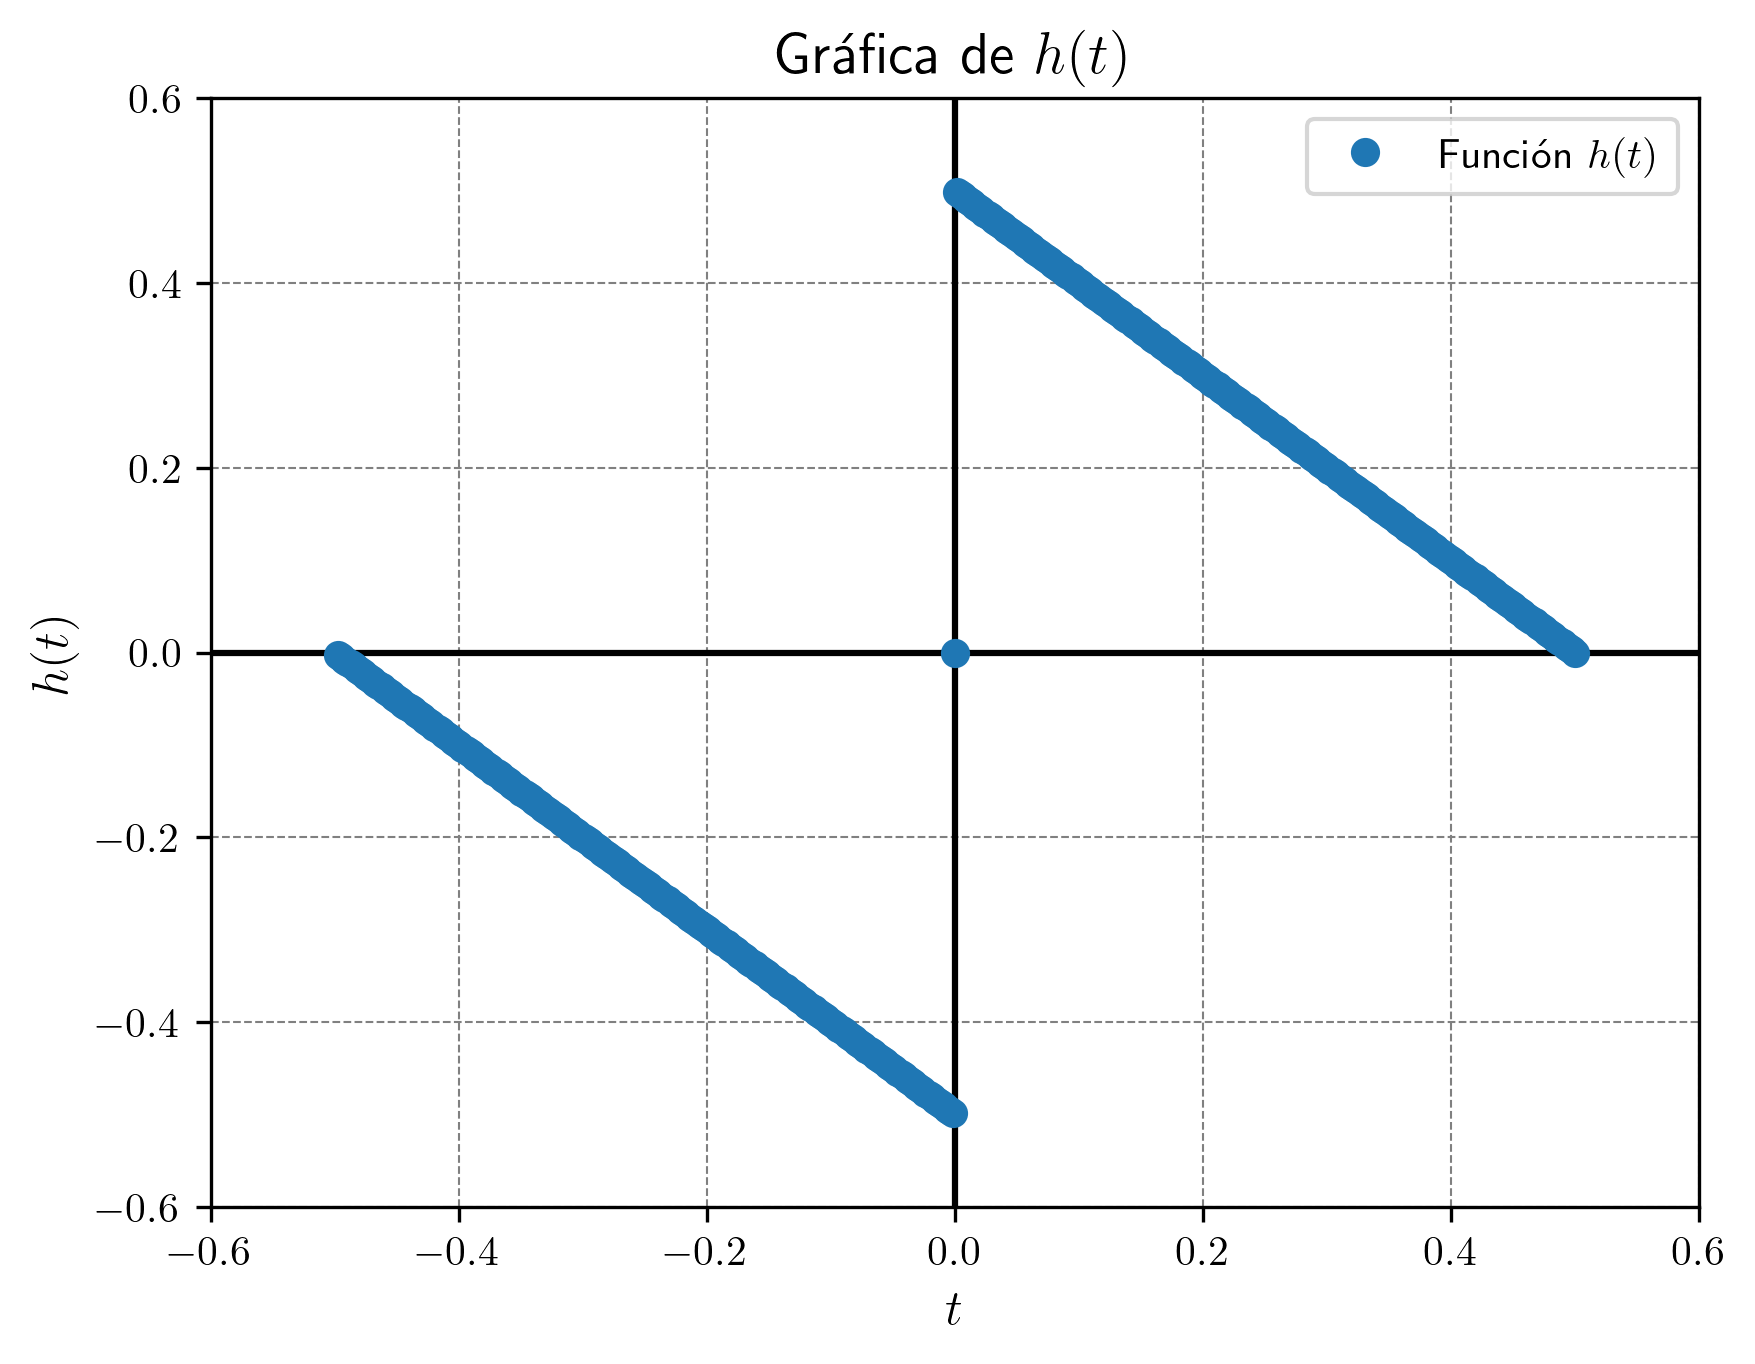
\includegraphics[scale=0.5]{Figures/h.png}
\end{center}
\end{figure}
Luego, es claro que $h$ es de variación acotada y continua excepto en el punto $t=0$, en dónde tiene una discontinuidad de salto. Además, note que $h$ es una función impar, por lo que podemos cálcular su transformada de Fourier de la siguiente manera:
\begin{equation}\label{eq:h_transformada}
  \begin{split}
    \hat{h}(m)&=\int_{\frac{-1}{2}}^{\frac{1}{2}}h(t)e^{-2\pi itm}dt,\\
    &=-2i \int_{0}^{\frac{1}{2}}\left( \frac{1}{2}-t \right)\sen(2\pi mt)dt,\\
    &=-\frac{i}{2m\pi}.  
  \end{split}
\end{equation}
Cuando $m\neq 0$ y por otro lado $\hat{h}(0)=0$.\\
Luego, las sumas parciales de Fourier de $h$ son:
\begin{equation}\label{eq:serie_h}
  \begin{split}    
    (h*D_{N})(t)&=-\frac{i}{2\pi}\sum_{\substack{|m| \leq N \\ m \neq 0}}\frac{e^{2\pi i mt}}{m}.
  \end{split}
\end{equation}
Ahora derivando respecto a $t$
\begin{equation}\label{eq:derivada_h}
  \begin{split}
    \frac{d}{dt}(h*D_{N})&=\sum_{\substack{|m| \leq N \\ m \neq 0}}e^{2\pi imt},\\
    &=D_{N}(t)-1.    
  \end{split}
\end{equation}
Siendo así, definamos $g(s)=\frac{1}{\sen(\pi s)}-\frac{1}{\pi s}$, luego utilizando el teorema fundamental del cálculo en $(\ref{eq:derivada_h})$ podemos afirmar que
\begin{equation}\label{eq:convolucion}
  \begin{split}
    (h*D_{N})(t)&=\int_{0}^{t}D_{N}(s)-1ds\\
    &=-t + \int_{0}^{t}D_{N}(s)ds\\
    &=-t + \int_{0}^{t}\frac{\sen((2N+1)\pi s)}{\sen(\pi s)}ds\\
    &=-t + \int_{0}^{t}\frac{\sen((2N+1)\pi s)}{\sen(\pi s)}-\frac{\sen((2N+1)\pi s)}{\pi s}+\frac{\sen((2N+1)\pi s)}{\pi s}ds\\
    &=-t + \int_{0}^{t}g(s)\sen((2N+1)\pi s)ds +\int_{0}^{t}\frac{\sen((2N+1)\pi s)}{\pi s}ds.
  \end{split}
\end{equation}
Además, se puede ver que
\begin{align*}
  \lim_{s \to 0}g(s)&=\lim_{s \to 0}\frac{1}{\sen(\pi s)}-\frac{1}{\pi s},\\
  &=\lim_{s \to 0}\frac{\pi s-\sen(\pi s)}{\sen(\pi s)\pi s},\\
  &=\lim_{u \to 0}\frac{u-\sen(u)}{\sen(u)u},\\
  &=\lim_{u \to 0}\frac{1-\cos(u)}{\cos(u)u+\sen(u)},\\
  &=\lim_{u \to 0}\frac{\sen(u)}{-\sen(u)u+2\cos(u)},\\
  &=\frac{0}{2},\\
  &=0.
\end{align*}
Por lo que podemos asegurar que $g$ es continua en $0$ y además $g(0)=0$, luego
\begin{align*}
  \lim_{s \to 0}\frac{g(s)}{s}&=\pi\lim_{u \to 0}\frac{u-\sen(u)}{\sen(u)u^2},\\
  &=\pi \lim_{u \to 0}\frac{1-\cos(u)}{\cos(u)u^2+2\sen(u)u},\\
  &=\pi \lim_{u \to 0}\frac{\sin(u)}{-\sen(u)u^2+4\cos(u)u+2\sen(u)},\\
  &=\pi \lim_{u \to 0}\frac{\cos(u)}{-\cos(u)u^2-6\sen(u)u+6\cos(u)},\\
  &=\frac{\pi}{6}.
\end{align*}
De esto que $g(s)$ sea continua y diferenciable en $[0,\frac{1}{2}]$ y $g'(0)=\frac{\pi}{6}$, además es claro que $g$ y $g'$ son funciones no negativas crecientes en el intervalo $[0,\frac{1}{2}]$, luego
\begin{align*}
  g'(s)&=\left( \frac{1}{\sen(\pi s)}-\frac{1}{\pi s} \right)',\\
  &=-\frac{\pi\cos(\pi s)}{\sen^2(\pi s)}+\frac{1}{\pi s^2},\\
  &\leq -\frac{\pi\cos(\pi/2)}{\sen^2(\pi/2)}+\frac{4}{\pi},\\
  &\leq \frac{4}{\pi}.
\end{align*}
Ahora, utilizando esto se sigue que
\begin{equation}\label{eq:O-grande-h}
  \begin{split}
    \left|\int_{0}^{t}g(s)\sen((2N+1)\pi s)ds\right|&=\left|-\frac{\cos((2N+1)\pi t)}{(2N+1)\pi}g(t)+\int_{0}^{t}g'(s)\frac{\cos((2N+1)\pi s)}{(2N+1)\pi}ds\right|,\\
    &\leq \left(g\left(\frac{1}{2}\right)+\frac{1}{2}g'\left(\frac{1}{2}\right) \right)\frac{1}{\pi}\frac{1}{2N+1},\\
    &\leq O\left( \frac{1}{2N+1} \right).
  \end{split}
\end{equation}
Luego, reemplazando $(\ref{eq:O-grande-h})$ en $(\ref{eq:convolucion})$ nos queda que
\begin{equation}\label{eq:6}
  \begin{split}
    (h*D_{N})(t)&=-t+\frac{1}{\pi}\int_{0}^{t}  \frac{\sen((2N+1)\pi s)}{s}ds+O\left( \frac{1}{2N+1} \right),\\
    &=-t+\frac{1}{\pi}\int_{0}^{(2N+1)\pi t}  \frac{\sen(s)}{s}ds+O\left( \frac{1}{2N+1} \right),\\
  \end{split}
\end{equation}
Ahora note que si tomamos $t\in(0,\frac{1}{2}]$, entonces $\lim_{N \to \infty}(h*D_N)(t))=-t+\frac{1}{\pi}\frac{\pi}{2}=\frac{1}{2}-t$, lo que se espera del núcleo de Dirichlet. De igual forma si tomamos $t\in[-\frac{1}{2},0)$, entonces $\lim_{N \to \infty}(h*D_N)(t)=-t-\frac{1}{\pi}\frac{\pi}{2}=-\frac{1}{2}-t$. También note que para $t=0$ se cumple que $\lim_{N \to \infty}(h*D_{N})(0)=0$, por lo que podemos ver que la serie de $h$ converge al promedio de $h(0+)$ y $h(0-)$, que resulta ser $h(0)=0$.\\
Con la intención de estimar la no uniformidad de la convergencia haremos lo siguiente
\begin{align*}
  (h*D_N)(t)-\left( \frac{1}{2}-t \right)&=\frac{1}{\pi}\int_{0}^{(2N+1)\pi t}\frac{\sen(s)}{s}ds-\frac{1}{2}+O\left( \frac{1}{2N+1} \right).
\end{align*}
luego si tomamos $N=1,2,\cdots$ y $t\in (0,\frac{1}{2}]$ se cumple rigurosamente que 
\begin{align*}
  (h*D_N)(t)-h(t)&\leq \frac{Si((2N+1)\pi)}{\pi}-\frac{1}{2}+\frac{1}{\pi}\frac{1}{2N+1},\\
  &\leq \frac{Si(\pi)}{\pi}-\frac{1}{2}+\frac{1}{\pi}\frac{1}{2N+1},\\
  &\leq 0.08949\cdots+\frac{\pi^{-1}}{2N+1}.
\end{align*}
Luego escogiendo una subsucesión $t_N\to 0$ nosotros tenemos que
\begin{equation}\label{eq:cota}
  \limsup_{N\to\infty}\left[ (h*D_{N})(t_{N})-h(t_{N}) \right]\leq \frac{Si(\pi)}{\pi}-\frac{1}{2}=0.08949\cdots,
\end{equation}
Luego, es particular si tomamos $t_N=\frac{1}{2N+1}$ se cumple que
\begin{align*}
  \limsup_{N\to\infty}\left[ (h*D_{N})(t_N)-h(t_{N}) \right]=\frac{Si(\pi)}{\pi}-\frac{1}{2}=0.08949\cdots
\end{align*}
Veamos esto gráficamente
\begin{figure}[H]
\begin{center}
  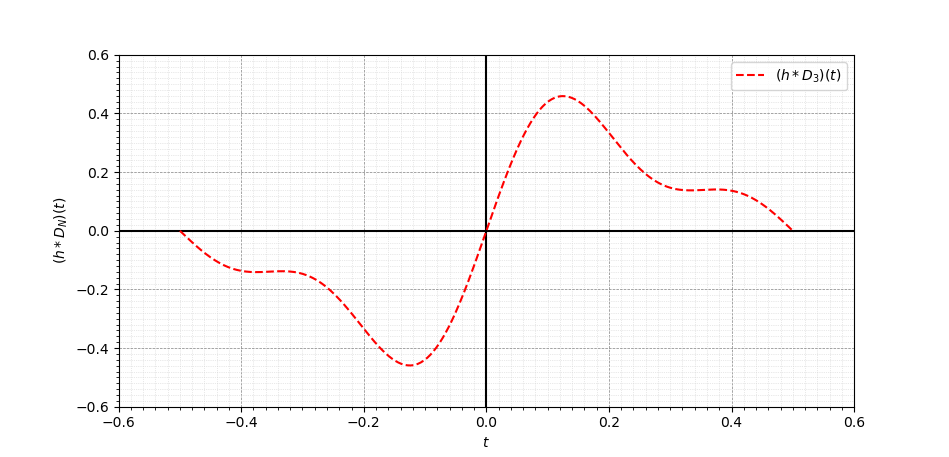
\includegraphics[scale=0.31]{Figures/3-serie.png}
  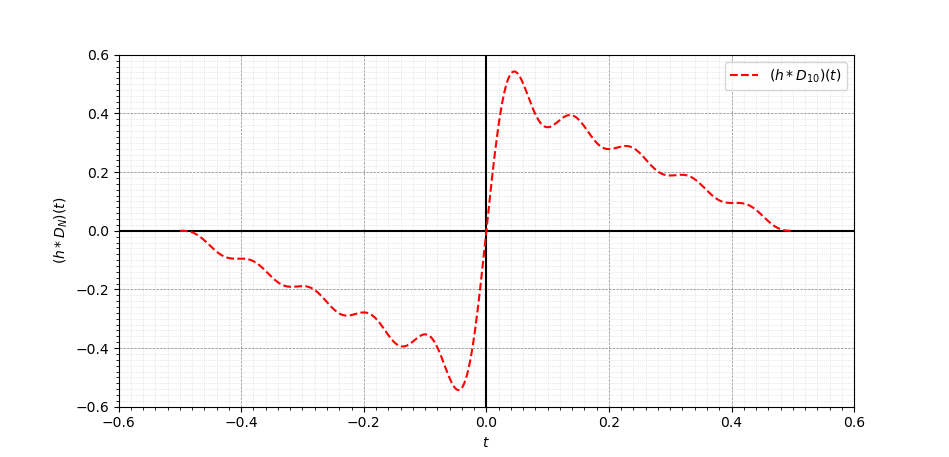
\includegraphics[scale=0.31]{Figures/10-serie.png}\\
  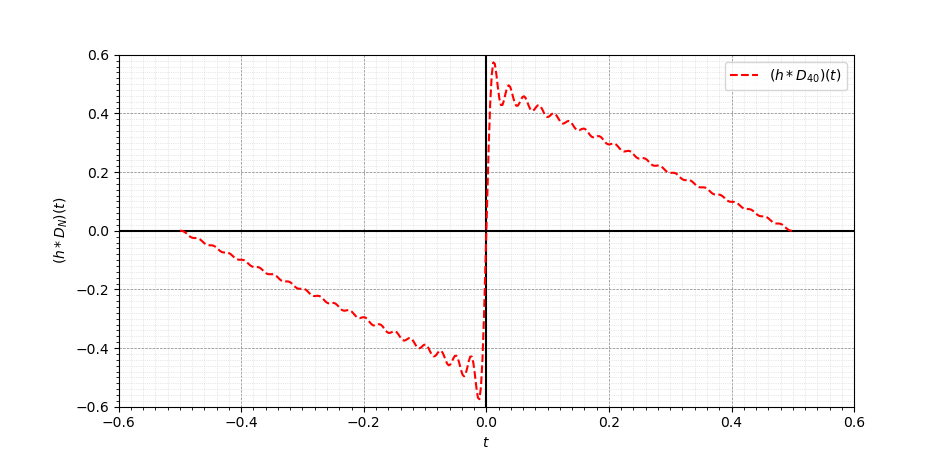
\includegraphics[scale=0.31]{Figures/40-serie.png}
  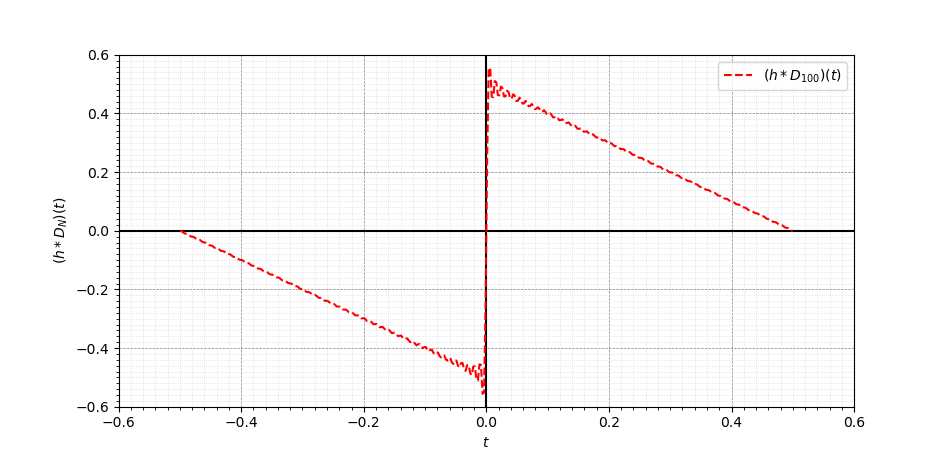
\includegraphics[scale=0.31]{Figures/100-serie.png}
\end{center}
  \caption{Series de Fourier $N=3,10,40$ y $100$.}
\label{fig:series-de-fourier-h}
\end{figure}
En dónde se puede ver que las series presentan un sobreimpulso de aproximadamente $9\%$ al acercarse al salto del $0$, a este suceso se le llama el fenómeno de Gibbs.\\
Ahora será interesante examinar el comportamiento de este fenómeno en el contexto de las funciones de variación acotada. Sabemos que las funciones de variación acotada pueden escribirse como resta de funciones crecientes, por lo que sabemos que estas tienen conjuntos a lo más un conjunto numerable de discontinuidades.\\
Siendo así, suponga $f\in L^{1}([-\frac{1}{2},\frac{1}{2}])$ de variación acotada y por simplicidad para la exposición supongamos que este solamente tiene $1$ discontinuidad de salto en un punto $t_0\in [-\frac{1}{2},\frac{1}{2}]$.
Ahora, utilizando la función $h$ dada en el ejemplo (\ref{eq:h}) muestra definamos
\begin{equation}\label{eq:f0}
  \begin{split}
    f_0(t)= 
    \begin{cases}
      \left( f(t_0+)-f(t_0-) \right)h(t-t_0)+\frac{f(t_0+)-f(t_0-)}{2}, &\text{ cuando } t\neq t_0 \text{,} \\
      f(t_0), &\text{ cuando } t=t_0.
    \end{cases}  
  \end{split}
\end{equation}
Ahora, note que si tomamos $t\in[-\frac{1}{2},\frac{1}{2}]$, entonces $f-f_0$ es de variación acotada, continua y cumple que $(f-f_0)(t_0)=0$, por lo que podemos afirmar que $((f-f_0)*D_{N})(t)\to (f-f_0)(t)$ uniformemente cuando $N\to \infty$ y por tanto la falta de uniformidad vista anteriormente se debe de presentar en el punto $t_0$.
Veamos el resultado en el siguiente teorema.
\begin{theorem}
  \begin{enumerate}
    \item Suponga $h$ como $(\ref{eq:h})$. Entonces el conjunto se puntos de acumulación de los conjuntos $\{(h*D_{N})(t_N)\}_{N\in\mathbb{Z}^{+}}$, donde $t_N\in[0,\frac{1}{2}]$, es el intervalo
      \begin{align*}
        \left[0,\frac{1}{2}\right]=[0,0.58949\cdots].
      \end{align*}
      En particular si $t_{N}\to 0$ tal que $Nt_{N}\to \frac{1}{2}$, entonces
      \begin{align*}
        \lim_{N \to \infty}(h*D_{N})(t_N)=\frac{Si(\pi)}{\pi}=0.58949\cdots
      \end{align*}
    \item Suponga $f$ como una función de variación acotada en $[-\frac{1}{2},\frac{1}{2}]$ con una discontinuidad de salto en el punto $t_0$, tal que $f(t_0+)-f(t_0-)>0$. Entonces el conjunto de puntos de acumulación de los conjuntos de la forma $\{(f*D_N)(t_N)\}_{N\in\mathbb{Z}^{+}}$, donde $t_N\in [t_0,t_0+\delta]$ para algún $\delta >0$, es el intervalo
      \begin{align*}
        \left[ \frac{f(t_0+)+f(t_0-)}{2},\frac{f(t_0+)+f(t_0+)}{2}+\frac{Si(\pi)}{\pi}(f(t_0+)-f(t_0-)) \right].
      \end{align*}
      En particular si $t_N\to t_0+$ tal que $N(t_N-t_0)\to\frac{1}{2}$, entonces
      \begin{align*}
        \lim_{N \to \infty}(f*D_{N})(t_N)=\frac{f(t_0+)+f(t_0+)}{2}+\frac{Si(\pi)}{\pi}(f(t_0+)-f(t_0-))
      \end{align*}
  \end{enumerate}
\end{theorem}
\begin{proof}
  \begin{enumerate}
    \item Dado que \( h \geq 0 \) en \( \left( 0, \frac{1}{2} \right] \) y \( (h * D_N)(t) \to \frac{1}{2} - t \) para \( 0 < t \leq \frac{1}{2} \), tenemos que todos los puntos de acumulación de las sucesiones \( (h * D_N)(t_N) \) son no negativos. Como vimos en el ejemplo que todos los puntos de acumulación de las sucesiones \( (h * D_N)(t_N) - h(t_N) \) son a lo sumo \( \frac{\operatorname{Si}(\pi)}{\pi} - \frac{1}{2} \); pero \( h(t_N) \leq \frac{1}{2} \), cuando \( t_N \in [0, \frac{1}{2}] \), por lo que todos los puntos de acumulación de las sucesiones \( (g * D_N)(t_N) \) son a lo sumo \( \frac{\operatorname{Si}(\pi)}{\pi} \) y, por lo tanto, están contenidos en \( \left[0, \frac{\operatorname{Si}(\pi)}{\pi} \right] \). Además, \( 0 \) se alcanza como punto de acumulación de \( (h * D_N)(0) \) y el número \( \frac{\operatorname{Si}(\pi)}{\pi} \) se alcanza como el punto de acumulación de la sucesión \( (h * D_N) \left( \frac{1}{2N+1} \right) \), como se muestro anteriormente.\\
      Note que la misma afirmación es válida para cualquier otra sucesión \( t_N \to 0 \) tal que \( N t_N \to \frac{1}{2} \).\\
      Ahora, dado que las funciones \( (h * D_N)(t) \) son continuas, dado cualquier \( c \in \left[0, \frac{\operatorname{Si}(\pi)}{\pi} \right] \), existe un \( t_N' \) entre \( 0 \) y \( \frac{1}{2N+1} \) tal que \( (h * D_N)(t_N') = c \) para todo \( N \), lo que muestra que el conjunto de puntos de acumulación de sucesiones de la forma \( \{(f * D_N)(t_N)\}_{N \in \mathbb{Z}^+} \) es el intervalo \( \left[0, \frac{\operatorname{Si}(\pi)}{\pi} \right] \).
    \item Para examinar el comportamiento de \( f * D_N \) cerca del punto de una única discontinuidad de salto \( t_0 \) de \( f \), reducimos el problema a la situación anterior mencionada anteriormente, introduciendo la función \( f_0 \) definida en (\ref{eq:f0}). Entonces, para una sucesión \( t_N \) que converge a \( t_0 \) por la derecha, tenemos
      \begin{align*}
      (f * D_N)(t_N) &= (f - f_0) * D_N(t_N) + (f(t_0+) - f(t_0-)) (h * D_N)(t_N - t_0) + \frac{f(t_0+) + f(t_0-)}{2} \\
      &= (f(t_0+) - f(t_0-)) \left[(h * D_N)(t_N - t_0) - h(t_N - t_0) \right] \\
      &\quad + (f(t_0+) - f(t_0-)) h(t_N - t_0) + (f - f_0) * D_N (t_N) + \frac{f(t_0+) + f(t_0-)}{2}.
      \end{align*}
      Aplicando \( \limsup_{N \to \infty} \) y usando la estimativa de uniformidad, obtenemos que cuando \( N \to \infty \),
      \[
      \limsup_{N \to \infty} (f * D_N)(t_N) \leq (f(t_0+) - f(t_0-)) \left( \frac{\operatorname{Si}(\pi)}{\pi} - \frac{1}{2} + \frac{1}{2} \right) + \frac{f(t_0+) + f(t_0-)}{2},
      \]
      donde usamos que $f-f_0$ es de variación acotada 
      \[
      \limsup_{N \to \infty} (f - f_0) * D_N(t_N) = (f - f_0)(t_0) = 0.
      \]
      Esto muestra que todos los puntos de acumulación de sucesiones de la forma \( \{(f * D_N)(t_N)\}_{N \in \mathbb{Z}^+} \) son como máximo \( (f(t_0+) - f(t_0-)) \frac{\operatorname{Si}(\pi)}{\pi} + \frac{1}{2} (f(t_0+) + f(t_0-)) \). Además, dado que todos los puntos de acumulación de sucesiones \( (g * D_N)(t_N) \) son no negativos, cuando \( t_N \) se encuentra a la derecha de \( t_0 \), se deduce de la identidad \( f = (f - f_0) + f_0 \) y (\ref{eq:f0}) que todos los puntos de acumulación de \( \{(f * D_N)(t_N)\}_{N \in \mathbb{Z}^+} \) son al menos \( \frac{1}{2} (f(t_0+) + f(t_0-)) \). Como en la parte (a), el teorema del valor intermedio implica que cada punto en el intervalo cuyos extremos son los mencionados anteriormente también es un punto de acumulación para la sucesión considerada.
  \end{enumerate}
\end{proof}



